\documentclass[aspectratio=169, 9pt]{beamer}

%%%%%%%%%%%%%%%%%%%%%%%%%%%%%%%%%%%%%%%%%%%%%%%%%%%%%%%%%%%%%%%%%%%%%%%%%
%%%%%%%%%%%%%%%%%%%%%%%%%%%%%%%%%%%%%%%%%%%%%%%%%%%%%%%%%%%%%%%%%%%%%%%%%

\usetheme{Copenhagen}
%\usecolortheme{seahorse}
\usefonttheme{professionalfonts}
\usepackage{palatino}

\usepackage{times}
\usepackage{hyperref}
\usepackage{tikz}
\usepackage{pgfplots}
\pgfplotsset{compat=1.18}
\pgfplotscreateplotcyclelist{worldlines}{{blue!80!black},{red!80!black},{black},{teal},{orange!90!black},{violet},{brown},{green!50!black},{magenta!80!black},{gray}}
% Worldlines q_1(t), ..., q_N(t) from the CSV files of the thesis (thesis/data)
\newcommand{\worldlines}[4]{% #1 file, #2 N, #3 width, #4 height
  \begin{tikzpicture}
  \begin{axis}[width=#3, height=#4, xlabel={$t$}, ylabel={$q$},
    enlarge x limits=false, tick label style={font=\tiny},
    label style={font=\scriptsize}, cycle list name=worldlines,
    every axis plot/.append style={line width=0.5pt, mark=none}]
  \pgfplotsinvokeforeach{1,...,#2}{\addplot table[x=t, y=q##1, col sep=comma]{#1};}
  \end{axis}
  \end{tikzpicture}}
\usepackage[english]{babel}
\usepackage{tcolorbox} % Allows boxes
\usepackage{graphicx} % Allows including images
\usepackage{booktabs}
\usepackage{amsmath}
%\usepackage{amsfonts}
\usepackage{amssymb}
\usepackage{subcaption}
\usepackage{siunitx}

%Maths Tools
\usepackage{amsmath}
\usepackage{amsthm}
\usepackage{amsfonts}
\usepackage{mathtools}
\usepackage{mathrsfs}
\usepackage{bbold}
\usepackage[overload]{empheq}

% Customized environments
\newtheorem{defi}{Definition}
\newtheorem{prop}{Proposition}
\newtheorem{thm}{Theorem}
\newtheorem{cor}{Corollary}
\newtheorem{obs}{Observation}

\newcommand{\diag}{\mathop{\mathrm{diag}}}
\DeclareMathOperator{\sech}{sech}

\setbeamertemplate{section in toc}[sections numbered]  % to create content list

\setbeamertemplate{caption}[numbered] % to number the captions

\setbeamerfont{caption}{size=\tiny} % Changes the font size of the captions
%\setbeamerfont{footnote}{size=\tiny} % Changes the font size of footnotes
\setbeamerfont{footline}{ size=\fontsize{7}{9}\selectfont}
\setbeamerfont{footnotemark}{size=\miniscule}
\setbeamertemplate{headline}{}

\setbeamertemplate{footline}{
\leavevmode%
\hbox{%
\begin{beamercolorbox}[wd=.333333\paperwidth,ht=2.25ex,dp=1ex,center]{author in head/foot}%
    \usebeamerfont{title in head/foot}\insertshortauthor
\end{beamercolorbox}%
\begin{beamercolorbox}[wd=.333333\paperwidth,ht=2.25ex,dp=1ex,center]{title in head/foot}%
    \usebeamerfont{title in head/foot}\insertshortinstitute
\end{beamercolorbox}%
\begin{beamercolorbox}[wd=.333333\paperwidth,ht=2.25ex,dp=1ex,right]{date in head/foot}%
    \usebeamerfont{date in head/foot}\insertshortdate{}\hspace*{2em}
    \insertframenumber{} / \inserttotalframenumber\hspace*{2ex} 
\end{beamercolorbox}}%
\vskip0pt%
}

\author[Andrea Zingarofalo ]{}
\date{November 11, 2022}
\title{\huge Soliton solutions \\
to classical Calogero-Moser systems}
\subtitle{} 
\institute[Scuola Superiore ISUFI] % (optional)
{
    \begin{columns}
    \begin{column}{0.5\textwidth}
    \begin{center}
    {\large \textit{\rmfamily Mentor:}} \\ \vspace{1.5 mm}
    {\large Prof. L. Martina} \vspace{5mm}
    \end{center}
    \end{column}
    \begin{column}{0.5\textwidth} 
    \begin{center}
    {\large \textit{\rmfamily Student:}} \\ \vspace{1.5 mm} {\large Andrea Zingarofalo} \vspace{5mm}
    \end{center}
    \end{column}
    \end{columns}
}


%%%%%%%%%%%%%%%%%%%%%%%%%%%%%%%%%%%%%%%%%%%%%%%%%%%%%%%%%%%%%%%%%%%%%%%%%%%%%%%%%%%
%   Main Document Starts Below

\begin{document}

%   Title Slide
{
\setbeamertemplate{footline}{
\leavevmode%
\hbox{%
\begin{beamercolorbox}[wd=.333333\paperwidth,ht=2.25ex,dp=1ex,center]{author in head/foot}%
    \usebeamerfont{title in head/foot}\insertshortauthor
\end{beamercolorbox}%
\begin{beamercolorbox}[wd=.333333\paperwidth,ht=2.25ex,dp=1ex,center]{title in head/foot}%
    \usebeamerfont{title in head/foot}\insertshortinstitute
\end{beamercolorbox}%
\begin{beamercolorbox}[wd=.333333\paperwidth,ht=2.25ex,dp=1ex,right]{date in head/foot}%
    \usebeamerfont{date in head/foot}\insertshortdate{}\hspace*{2em}
%    \insertframenumber{} / \inserttotalframenumber\hspace*{2ex} 
\end{beamercolorbox}}%
\vskip0pt%
}
\begin{frame}
    \begin{center}
            \begin{minipage}[c]{0.2\linewidth}
                    \begin{center}
                    
\includegraphics[width=2.5 cm, height=1.3 cm]{./Graphics/Logo_ISUFI.png} 
                    \end{center}
            \end{minipage}
            \begin{minipage}[c]{0.5\linewidth}
                    \begin{center}
                    \begin{large}
                   \rmfamily Scuola Superiore ISUFI\\ \vspace{1mm} Curriculum Tecnico-Scientifico
                    \end{large} 
                    \end{center}
            \end{minipage}
    \end{center}
\titlepage
\end{frame}
}

%%%%%%%%%%%%%%%%%%%%%%%%%%%%%%%%%%%%%%%%%%%%%%%%%%%%%%%%%%%%%%%%%%%%%%%%

\begingroup 
    \setbeamertemplate{headline}{}
    \addtobeamertemplate{frametitle}{\vspace*{-\headheight}}{}
    \begin{frame}{Outline}
        \tableofcontents{}
    \end{frame}
\endgroup

%%%%%%%%%%%%%%%%%%%%%%%%%%%%%%%%%%%%%%%%%%%%%%%%%%%%%%%%%%%%%%%%%%%%%%
% You Main Presentation Starts Here}

\section{Basic references}
\begin{frame}{Some basic references}
\nocite{*}
\bibliographystyle{unsrt}
\bibliography{references}      
\end{frame}


\section{Background: integrable systems}
\begin{frame}{Background: integrable systems}
\subsection{Introduction to integrability}
The field of integrable systems was born together with classical mechanics, with a quest for exact solutions to Newton's equations of motion. Two centuries after Newton's solution of the Kepler problem, only a few other cases were known:

\vspace{\baselineskip}

\begin{itemize}
    \item geodesics on the ellipsoid (Jacobi, 1838);
    \item the harmonic oscillator on the sphere (Neumann, 1859);
    \item Lagrange, Euler and Kovalevskaya tops.
\end{itemize}

\end{frame}

\subsection{Lax representation of an integrable system}
\begin{frame}[allowframebreaks]{Lax representation of an integrable system}

\begin{defi}
A Lax pair $(L,M)$ consists of two square matrices, functions on the phase space of the system, such that the Hamiltonian evolution equations may be written as

\begin{equation}\label{laxevolution}
\dot L = [L, M]
\end{equation}

where $[L,M]$ denotes the commutator on the set of matrices. 
\end{defi}

Suppose that $\mathcal{H}$ is integrable, and that the integrals of motion $\mathcal{H}_1, ..., \mathcal{H}_N$ are known. Then

\[ \hat L = \diag{ \{\mathcal{H}_i : i=1,...,N \}} \]

is a Lax representation of $\mathcal{H}$.
\end{frame}

\begin{frame}{Lax representation of an integrable system II}
Because similarity transformations preserve eigenvalues, if

\[L = U \hat LU^{-1}\]

where $U(t)$ is some invertible matrix, then the eigenvalues $\lambda_i$ of $L$ coincide with the ones of $\hat L$: $\lambda_i = \mathcal{H}_i$ ($i=1, \dots, N$). Consider now the eigenvalue equation

\[Lu_i = \lambda_i u_i\;.\]

Taking the time derivative we get:

\[\dot L u_i + L \dot u_i = \dot \lambda_i u_i + \lambda_i \dot u_i = \lambda_i \dot u_i\;.\]

Supposing $\dot u_i = - M u_i$, where $M \in \mathbb{C}^{\;N\times N}$ we have

\[\dot L u_i - LMu_i = -\lambda_i M u_i = - M \lambda_i u_i = - MLu_i\;,\]

thus

\[\dot L u_i - LMu_i = -MLu_i \iff (\dot L - [L,M])u_i = 0\;\;.\]

\[\implies \dot L = [L,M]\;.\]
\end{frame}

\begin{frame}{Lax representation of an integrable system III}
\begin{example}
A Lax pair for the harmonic oscillator has the form:

\[L = 
\begin{pmatrix}   
p & \omega q\\   
\omega q & -p  
\end{pmatrix},\;\;\;
M = 
\begin{pmatrix}   
0 & \frac{\omega}{2}\\   
-\frac{\omega}{2} & 0  
\end{pmatrix}\;.\]

The characteristic equation

\begin{equation}
    (p-\lambda) (p + \lambda) + \omega^2 q^2 = 0
\end{equation}

gives the eigenvalues

\begin{equation}
    \lambda_{1,2} = \pm \sqrt{p^2 + \omega^2 q^2}\;,
\end{equation}

that are integrals of motion of the system related to the energy. \\
We check immediately that $\dot L = [L, M]$ is equivalent to the equations of motion

\[\dot q = p, \;\;\;\;\;\;\;\;\dot p = -\omega^2 q\;\;\,.\]
\end{example} 
\end{frame}

\section{Calogero-Moser systems}
\begin{frame}[allowframebreaks]{Calogero-Moser systems}
\begin{defi}
Let $(q, p) = (q_1, \dots, q_N, p_1, \dots, p_N)$ be a set of canonical coordinates. A dynamical system is said to be an $A_{N-1}$ Calogero-Moser \textnormal{(CM)} system with some external potential $W(x)$ if it is characterized by the Hamiltonian

\begin{equation}
\mathcal{H}_{CM} = \sum_{i=1}^N \Big(\frac{1}{2} p_i^2 + W(q_i)\Big) + g^2 \sum_{1 \leq i < j \leq N} V(q_i - q_j)\;,
\end{equation}

(with unit masses), where $g^2$ is the coupling constant and the interparticle potential $V (x)$ belongs to the classified set of meromorphic functions

\[V(x) = \left \{ \begin{array}{ccc}
{1}/{x^2} & \textnormal{(rational)} & \textnormal{(I)}\\
{a^2}/{\sin^2{ax}} & \textnormal{(trigonometric)} & \textnormal{(II)}\\
{a^2}/{\sinh^2{ax}} & \textnormal{(hyperbolic)} & \textnormal{(III)}\\
\wp (x) & \textnormal{(elliptic)} & \textnormal{(IV)}
\end{array}
\right.\]

where $\wp (x)$ is the \textit{elliptic, doubly periodic Weierstrass function} with periods $2\omega_1$ and $2\omega_2$.
\end{defi}

\begin{itemize}
\item These forms of the potential are fixed by the form of the Lax pair proposed by F. Calogero. The general solution is given by the Weierstrass function $\wp(x)$, and the types I--III are its limiting cases:

\begin{equation}
    \wp(x) = \left \{ \begin{array}{ccc}
    {1}/{x^2} & \omega_1 = \infty & \omega_2 = \infty\\
    {a^2}/{\sin^2{ax}} - {a^2}/{3} & \omega_1 = {\pi} / {2a} & \omega_2 = i\infty\\
    {a^2}/{\sinh^2{ax}} + {a^2}/{3} & \omega_1 = \infty\ & \omega_2 = {i\pi}/{2a}
\end{array}
\right.
\end{equation}

\item From Hamilton's equations we get

\begin{equation}
    \ddot q_i = - W'(q_i) - g^2 \sum_{j = 1,\;j \neq i}^N V'(q_i - q_j)\;.
\end{equation}
\end{itemize}
\end{frame}

\subsection{KKS construction of CM systems}
\begin{frame}{KKS construction of CM systems}
In the Kazhdan-Kostant-Sternberg (KKS) construction of CM systems, CM systems emerge from Hamiltonians on the larger configuration space $X^0_N = \{X\}$ of $N \times N$ Hermitian matrices $X$. \\
If $U$ is unitary, then the Hamiltonians are invariant with respect to similarity transformations

\begin{equation}
    (X, Y) \mapsto (UXU^{-1}, UYU^{-1})\;.
\end{equation}

Introducing the $N \times N$ Hermitian matrices

\begin{equation}
\begin{cases}
Q_{nm} = \delta_{nm} q_n(t) \\
L_{nm} = \delta_{nm}p_n(t) + (1 - \delta_{nm}) \frac{ig}{q_n - q_m}\;,
\end{cases}
\end{equation}

such matrices correspond to generic Hermitian matrices $X, Y \in X_N^0$:

\begin{equation}
    X = UQU^{-1}\;\;\;\;,\;\;\;\;Y = ULU^{-1}\;.
\end{equation}
\end{frame}

\begin{frame}{KKS construction of the $\textnormal{I}^+$ system}
The KKS construction of the rational CM system with external harmonic potential starts from the Hamiltonian

\begin{equation}
    \mathcal{H}_{eCM} = \frac{1}{2}\operatorname{tr}(Y^2 + \omega^2 X^2), \;\;\;\;\;\;(X,Y) \in \mathcal{T}^\ast X^0_N\;.
\end{equation}

Applying the similarity transformation we get

\begin{equation}
\begin{split}
    \mathcal{H}_{eCM} &= \frac{1}{2}\operatorname{tr}(Y^2) + \frac{1}{2}\omega^2 \operatorname{tr}(X^2) = \\  &= \frac{1}{2}\operatorname{tr}(UU^{-1}Y^2) + \frac{1}{2}\omega^2 \operatorname{tr}(UU^{-1} X^2) = \\ 
    & = \frac{1}{2}\operatorname{tr}(U^{-1} Y^2 U) + \frac{1}{2}\omega^2 \operatorname{tr}(U^{-1} X^2 U)= \frac{1}{2}\operatorname{tr}(L^2) + \frac{1}{2}\omega^2 \operatorname{tr}(Q^2)\;.
\end{split}
\end{equation}

The projection then gives
    
\begin{equation}
    \mathcal{H}_{eCM} = \frac{1}{2}\operatorname{tr}(L^2) + \frac{1}{2}\omega^2 \operatorname{tr}(Q^2)= \frac{1}{2}\sum_{i=1}^N (p_i^2 + \omega^2 q_i^2) + g^2 \sum_{1 \leq i < j \leq N} \frac{1}{(q_i - q_j)^2}\;.
\end{equation}
\end{frame}

\subsection{The Olshanetsky-Perelomov projection method}
\begin{frame}{The Olshanetsky-Perelomov projection method}
Integrating the equations of motion of these systems directly is hard. However, an alternative method of integration has been developed by M. A. Olshanetsky and A. M. Perelomov. Their projection method amounts to the integration of the auxiliary Hamiltonian systems, from which the solution to the considered ones can be recovered by projection.
\end{frame}

\begin{frame}[allowframebreaks]{OP projection for $\textnormal{I}^+$ system}
From harmonic motion on $X^0_N$, described by the Hamiltonian

\begin{equation}
    \mathcal{H} = \frac{1}{2}\operatorname{tr}(Y^2 + \omega^2 X^2), \;\;\;\;\;\;(X,Y) \in \mathcal{T}^\ast X^0_N\;.
\end{equation}

we obtain the equation of motion $\ddot X + \omega^2 X= 0$, which integrates directly to 

\begin{equation}
    X = \frac{A}{\omega}\sin{\omega t} + B\cos{\omega t}\;\;\;\;,\;\;\;\;A, B \in X^0_N\;.
\end{equation}

If $X(t) = U(t) Q(t) U^{-1}(t)$, 

\[U(0) = \mathbb{1}_N \implies B = X(0) = Q(0)\;\;\;\;, \;\;\;\;A = \dot X(0) = L(0).\] 

Then,

\begin{equation}
    X_{nm} (t) = \delta_{nm} (p_n(0)\frac{\sin{\omega t}}{\omega} + q_n(0)\cos{\omega t}) + (1 - \delta_{nm}) ig \frac{\sin{\omega t}}{\omega(q_n(0) - q_m(0))}\;.
\end{equation}

And the time evolution of $Q(t)$ is given by

\begin{equation}
    Q(t) = U^{-1}(t) X(t) U(t)\;.
\end{equation}
\end{frame}

\subsection{Bäcklund transformations of CM systems}
\begin{frame}[allowframebreaks]{Bäcklund transformations of CM systems}
We introduce Bäcklund transformations (BTs) of CM systems, in a single form for I, II, III and $\textnormal{I}^+$.

\begin{thm}
Consider $N$ complex canonical coordinates $x_j = q_j, \dot x_j = p_j \in \mathbb{C}$ and $M$ canonical coordinates $z_n, \dot z_n \in \mathbb{C}$. Then, the Bäcklund transformations for CM systems of type $\textnormal{I,II,III}$ and $\textnormal{I}^+$ take the form

\begin{subequations}
\begin{align}[left=\empheqlbrace]
\dot x_j &= - \sum_{k=1,\;k \neq j}^N \alpha(x_j - x_k) + \sum_{n = 1}^M \alpha(x_j - z_n) + \lambda + i\omega x_j\;,\\
\dot z_n &= \sum_{m=1,\;m \neq n}^M \alpha(z_n - z_m) - \sum_{l = 1}^N \alpha(z_n - x_l) + \lambda + i\omega z_n\;,
\end{align}
\end{subequations}

with $\alpha(x)$ the \textit{special Lax function}, with the property $V(x) = - \alpha^2(x)$, $\lambda$ a constant and $\omega = 0$ for all but class $\textnormal{I}^+$.
\end{thm}
\end{frame}

\section{Soliton solutions to Calogero-Moser systems}
\subsection{Poles of nonlinear waves as interacting particles}
\begin{frame}[allowframebreaks]{Poles of nonlinear waves as interacting particles}
Consider the Benjamin-Ono equation

\begin{equation}\label{benjaminono}
    u_t + \hat H u_{xx} + 2uu_x = 0\;,
\end{equation}

where $\hat H$ is the Hilbert transform

\begin{equation}
    \hat H[f](x) = \frac{\textnormal{p.v.}}{\pi}\int_{- \infty}^{+ \infty} \frac{f(z)}{x - z}dz\;,
\end{equation}

with $\textnormal{p.v.}$ the Cauchy principal value. This model describes internal waves of permanent form in a deep fluid. 

\begin{figure}
    \centering
    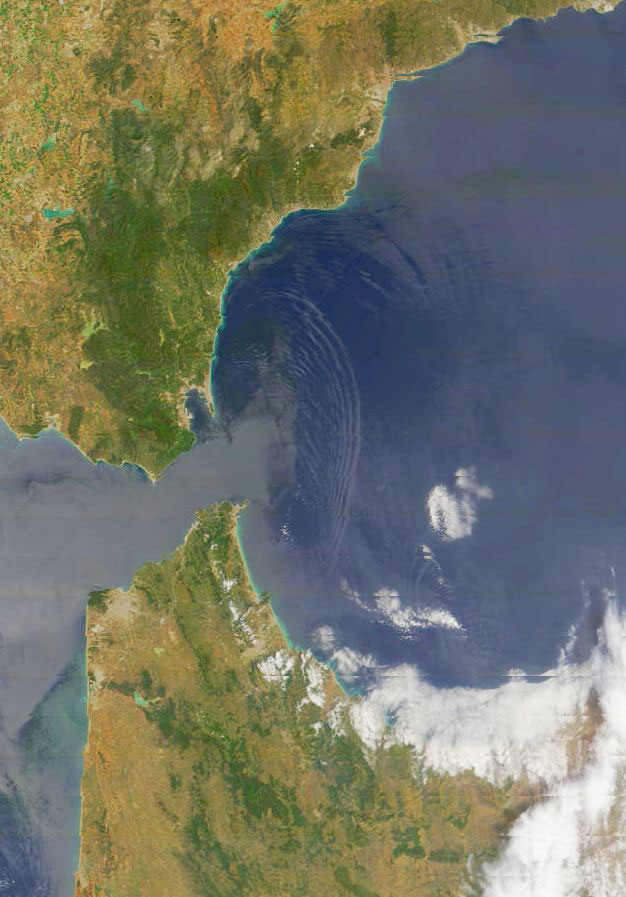
\includegraphics[width = 4cm]{images/internalwavesgibraltar.jpg}
    \caption{Internal waves in the Eastern Strait of Gibraltar (source: EUMETSAT).}
\end{figure}
\end{frame}

\begin{frame}{Poles of nonlinear waves as interacting particles III}
A solution of the BO equation has the form

\begin{equation}
    u(x,t) = i\sum_{n=1}^N \Big ( \frac{1}{x - z_n(t)} - \frac{1}{x - z_n^\ast (t)} \Big )\;,
\end{equation}

whose poles satisfy the complex Calogero-Moser equations of motion

\begin{equation}
    \ddot z_n(t) = 8 \sum_{m=1,\;m \neq n}^N \frac{1}{(z_n(t) - z_m(t))^3}\;.
\end{equation}
\end{frame}

\begin{frame}{Poles of nonlinear waves as interacting particles IV}
The following holds.

\begin{thm}
Let $\alpha(x)$ be a special Lax function. The meromorphic functions 

\begin{equation}\label{solitonequation}
    u(x,t) = \sum_{j=1}^N \alpha (x - x_j) - \sum_{n=1}^M \alpha (x - z_n) - i\omega x\;,
\end{equation}

for arbitrary $N$ and $M$ form a class of solutions to equations of Benjamin-Ono type (the equation (\ref{benjaminono}) itself in the rational case with $\omega = 0$) if and only if their poles $\{x_j\}$ and $\{z_n\}$ satisfy the system of equations

\begin{subequations}
\begin{align}[left=\empheqlbrace]
\dot x_j &= - \sum_{k=1,\;k \neq j}^N \alpha(x_j - x_k) + \sum_{n = 1}^M \alpha(x_j - z_n) + \lambda + i\omega x_j\;,\\
\dot z_n &= \sum_{m=1,\;m \neq n}^M \alpha(z_n - z_m) - \sum_{l = 1}^N \alpha(z_n - x_l) + \lambda + i\omega z_n\;,
\end{align}
\end{subequations}

where $\lambda$ and $\omega$ are constants. 
\end{thm}
\end{frame}

\begin{frame}{Poles of nonlinear waves as interacting particles V}

\begin{itemize}
\item We can operate a finite-dimensional reduction of such infinite-dimensional systems. Given a solution of the form $u(x,t)$ we can consider a discretization $u(x; \{z_n\})$ so that the time dependence of $u$ is reduced to $M$ complex parameters $z_n (t)$, with $n = 1, 2,..., M$ with known time dependence. 

\vspace{\baselineskip}

\item We call $u(x, \{z_n(t)\})$ for $n = 1, ..., M$ an $M$-soliton solution.
\end{itemize}
\end{frame}



\subsection{General method}
\begin{frame}[allowframebreaks]{General method}
Consider $N$ complex canonical coordinates $x_j = q_j, \dot x_j = p_j \in \mathbb{C}$ and $M$ canonical coordinates $z_n, \dot z_n \in \mathbb{C}$ and their respective Hamiltonians

\begin{subequations}
\begin{align}
    \mathcal{H} &= \frac{1}{2}\sum_j ({\dot x_j}^2 + \omega^2 x_j^2) + \sum_{j < k} V(x_j - x_k), \\
    \mathcal{H'} &= \frac{1}{2}\sum_n ({\dot z_n}^2 + \omega^2 z_n^2) + \sum_{n < m} V(z_n - z_m)\;.
\end{align}
\end{subequations}

Writing the special Lax function as $i\alpha(x)$, with $\alpha$ real on the real axis, a subset of the solutions to each system can be connected by a BT of the form

\begin{subequations}
\begin{align}[left=\empheqlbrace]
\dot x_j &= - i\sum_{k=1,\;k \neq j}^N \alpha(x_j - x_k) + i\sum_{n = 1}^M \alpha(x_j - z_n) + i\omega x_j \label{soliton1}\;,\\
\dot z_n &= i\sum_{m=1,\;m \neq n}^M \alpha(z_n - z_m) - i\sum_{l = 1}^N \alpha(z_n - x_l) + i\omega z_n\label{soliton1b}\;.
\end{align}
\end{subequations}

For $M < N$, the principal system is reduced via BTs into a system with fewer degrees of freedom. If $x_j, p_j = \dot x_j \in \mathbb{R} \;\forall j$ (real reduction), splitting (\ref{soliton1}) into its real and imaginary parts we get

\begin{subequations}
\begin{align}[left=\empheqlbrace]
    \sum_{k=1,\;k \neq j}^N \alpha (x_j - x_k) &= \sum_{n=1}^M \operatorname{Re}{\alpha(x_j - z_n)} + \omega x_j \label{soliton2}\;, \\
    \dot x_j &= - \sum_{n = 1}^M \operatorname{Im}{\alpha(x_j - z_n)} \label{soliton3}\;.
\end{align}
\end{subequations}

For $M$ given initial conditions $\{z_n(0)\}$, one can find both $N$ real positions $\{x_j(0)\}$ solving numerically (\ref{soliton2}), and the corresponding real momenta $\{\dot x_j(0)\}$ using (\ref{soliton3}). Then, the evolutions of the soliton solutions are determined by the OP projection.
\end{frame}

\subsection{1-soliton solutions for the eCM system}
\begin{frame}[allowframebreaks]{1-soliton solutions for the $\textnormal{I}^+$ system}
Solving the system numerically for the $\textnormal{I}^+$ system, we get the worldlines of the real system.

\begin{figure}[H]
    \centering
    \worldlines{../thesis/data/fig3_2.csv}{10}{8cm}{5cm}
    \caption{Worldlines of the real $\textnormal{I}^+$ system for $N = 10$ particles, with $\omega = g = 1$ and initial value $z(0) = 1 + i$.}
    \label{fig:my_label}
\end{figure}

The soliton wave propagates along the real axis in coordination with the complex orbit $z(t)$. The soliton wave appears to propagate with constant speed (the shifts appear to be regularly spaced in time). The soliton excitation corresponds to the upward or downward shifts in the worldlines.  

\begin{figure}[H]
\centering
\begin{subfigure}{.5\textwidth}
  \centering
  \worldlines{../thesis/data/fig3_3a.csv}{10}{6cm}{4.2cm}
  \caption{}
  \label{fig:sub1}
\end{subfigure}%
\begin{subfigure}{.5\textwidth}
  \centering
  \worldlines{../thesis/data/fig3_3b.csv}{10}{6cm}{4.2cm}
  \caption{}
  \label{fig:sub2}
\end{subfigure}
\caption{Worldlines of the real $\textnormal{I}^+$ system for $N = 10$ particles, with $\omega = g = 1$ and initial values $z(0) = 1.2 + 0.3i$ for \ref{fig:sub1} and $z(0) = 2.8 + 2.4i$ for \ref{fig:sub2}.}
\label{fig:test}
\end{figure}

In Figure~\ref{fig:test} we can observe that if $z(0)$ is closer to the real axis, it yields a tighter orbit and more pronounced wave, while $z(0)$ farther gives the opposite behaviour.
\end{frame}

\subsection{$M$-soliton solutions for the eCM system}
\begin{frame}[allowframebreaks]{$M$-soliton solutions for the $\textnormal{I}^+$ system}

We can apply the general method to the rational potential with external harmonic potential (eCM) for a generic $M < N$:

\begin{subequations}
\begin{align}[left=\empheqlbrace]
\dot x_j &= -ig \sum_{k=1,\;k \neq j}^N \frac{1}{(x_j - x_k)} + ig \sum_{n = 1}^M \frac{1}{(x_j - z_n)} + i\omega x_j \label{soliton7}\;,\\
\dot z_n &= ig \sum_{m=1,\;m\neq n}^M \frac{1}{z_n - z_m} - ig \sum_{l=1}^N \frac{1}{(z_n - x_l)} + i\omega z_n\;.
\end{align}
\end{subequations}

Separating (\ref{soliton7}) into its real and imaginary parts, we get

\begin{subequations}
\begin{align}[left=\empheqlbrace]
    \omega x_j &= g\sum_{k=1,\;k \neq j}^N \frac{1}{x_j - x_k} - g \sum_{n=1}^M\operatorname{Re}{\frac{1}{x_j - z_n}} \label{soliton8}\;, \\
    \dot x_j &= - g \sum_{n=1}^M\operatorname{Im}{\frac{1}{x_j - z_n}} \label{soliton9}\;.
\end{align}
\end{subequations}

Solving numerically (\ref{soliton8}) for $\{z_n(0)\}$, $n = 1, \dots, M$, we find the $N$ positions $\{x_j(0)\}$, and then $\{\dot x_j(0)\}$ using (\ref{soliton9}). \\
The evolutions of the soliton solutions $\{x_j(t)\}$ and $\{z_n(t)\}$ are given by the eigenvalues of

\begin{subequations}
\begin{align}
    X_{jk} (t) &= \delta_{jk} \Big (\dot x_j(0)\frac{\sin{\omega t}}{\omega} + x_j (0)\cos{\omega t} \Big ) \nonumber\\ &\quad + (1 - \delta_{jk}) ig \frac{\sin{\omega t}}{\omega(x_j(0) - x_k(0))}\;, \\
    Z_{nm} (t) &= \delta_{nm} \Big (\dot z_n(0)\frac{\sin{\omega t}}{\omega} + z_n (0)\cos{\omega t} \Big ) \nonumber\\ &\quad + (1 - \delta_{nm}) ig \frac{\sin{\omega t}}{\omega(z_n(0) - z_m(0))}\;.
\end{align}
\end{subequations}

\begin{figure}[H]
\centering
\begin{subfigure}{.5\textwidth}
  \centering
  \worldlines{../thesis/data/fig3_4a.csv}{6}{6cm}{4.2cm}
  \caption{}
  \label{2soliton61}
\end{subfigure}%
\begin{subfigure}{.5\textwidth}
  \centering
  \worldlines{../thesis/data/fig3_4b.csv}{6}{6cm}{4.2cm}
  \caption{}
  \label{2soliton62}
\end{subfigure}
\caption{Worldlines of the real $\textnormal{I}^+$ system for $N = 6$ particles, with $\omega = g = 1$ and initial values $z_1(0) = -1.1 + 0.5i, z_2(0) = 0.1 -2i$ for \ref{2soliton61} and $z_1(0) = -1.1 + 0.5i, z_2(0) = 0.1 - i$ for \ref{2soliton62}.}
\end{figure}

For $M > 1$, we can note the effects of interaction between multiple solitons. The trajectories are deformed more or less significantly depending on the degrees of freedom of the dual system and the initial conditions.  

\begin{figure}[H]
\centering
\begin{subfigure}{.5\textwidth}
  \centering
  \worldlines{../thesis/data/fig3_5a.csv}{6}{6cm}{4.2cm}
  \caption{}
  \label{2soliton63}
\end{subfigure}%
\begin{subfigure}{.5\textwidth}
  \centering
  \worldlines{../thesis/data/fig3_5b.csv}{6}{6cm}{4.2cm}
  \caption{}
  \label{2soliton64}
\end{subfigure}
\caption{Worldlines of the real $\textnormal{I}^+$ system for $N = 6$ particles, with $\omega = g = 1$ and initial values $z_1(0) = 0.1 + 0.5i, z_2(0) = 0.1 -0.9i$ for \ref{2soliton63} and $z_1(0) = 0.1 + 0.5i, z_2(0) = 0.1 - 0.1i$ for \ref{2soliton64}.}
\end{figure}

\begin{figure}[H]
    \centering
    \worldlines{../thesis/data/fig3_6.csv}{10}{9cm}{5.2cm}
    \caption{Worldlines of the real $\textnormal{I}^+$ system for $N = 10$ particles, with $\omega = g = 1$ and initial values $z_1(0) = 0.1 + 0.5i, z_2(0) = 0.1 - i$.}
    \label{figsoliton10}
\end{figure}
\end{frame}

\subsection{Electrostatic interpretation}
\begin{frame}[allowframebreaks]{Electrostatic interpretation}
\begin{obs}
As is known in the literature, soliton solutions to the rational CM system correspond to extremal conditions of an electrostatic energy function $E$. In fact, considering the Coulomb potential $V(x_j - z_n) = \ln{|x_j - z_n|} = \frac{1}{2}\big[\ln{(x_j - z_n)} + \ln{(x_j - \bar z_n)}\big]$, we get

\begin{equation}
    \frac{\partial V(x_j - z_n)}{\partial x_j} = \frac{1}{2} \Big ( \frac{1}{x_j - z_n} + \frac{1}{x_j - \bar z_n} \Big ) = \operatorname{Re}{\frac{1}{x_j - z_n}}\;.
\end{equation}

Then, given $E$ the potential of the system

\begin{equation}
    E = \sum_{j=1}^N \frac{\omega x_j^2}{2} - g \sum_{1 \leq j < k \leq N} \ln{|x_j - x_k|} + \frac{g}{2} \sum_{j = 1}^N \sum_{n=1}^M \ln{|x_j - z_n|^2}\;,
\end{equation}

it follows

\begin{equation}
    \frac{\partial E}{\partial x_j} = \omega x_j - g \sum_{k=1,\;k \neq j}^N \frac{1}{x_j - x_k} + g\sum_{n=1}^M \operatorname{Re}{\frac{1}{x_j - z_n}}\;.
\end{equation}
\end{obs}

\begin{obs}
Hence, equation (\ref{soliton8}) can be derived from the extremal condition 

\begin{equation}
    \frac{\partial E}{\partial x_j} = 0\;.
\end{equation}

In this view, the positive charges $\{z_n\}$ interact with the negative charges $\{x_j\}$ on the line, inducing the soliton wave. 
\end{obs}
\end{frame}

\end{document}